\documentclass[a4paper,11pt]{article}
\newtheorem{thm}{Theorem}
\setlength{\oddsidemargin}{0.25in}
\setlength{\textwidth}{6in}
\setlength{\topmargin}{-0.25in}
\setlength{\headheight}{0.3in}
\setlength{\headsep}{0.2in}
\setlength{\textheight}{9in}
%\setlength{\footskip}{0.1in}
\usepackage{multirow}
\usepackage{fullpage}
\usepackage{graphicx}
\usepackage{amsthm}
\usepackage{amssymb}
\usepackage{url}
\usepackage{amsfonts}
\usepackage{algpseudocode}
\usepackage{mathtools}
\newcommand{\quotes}[1]{``#1''}

\usepackage{hyperref}
\hypersetup{
    colorlinks=true,
    linkcolor=blue,
    filecolor=magenta,      
    urlcolor=blue,
}


% ===== ===== ===== ===== ===== % 
% New commands set by Chuck Jia
% ===== ===== ===== ===== ===== % 

\newcommand{\code}[1]{\texttt{#1}}
\newcommand{\qnum}[1]{\noindent\textcolor{blue}{\textbf{(#1)}}}
\newcommand{\ds}{\displaystyle}
\newcommand{\sep}{\begin{center}\textcolor{gray}{\rule{\textwidth}{0.75pt}}\end{center}}
\usepackage{minted}



\begin{document}\title{Homework 1\\ Applied Machine Learning \\ Fall 2017\\ CSCI-P 556/INFO-I 526}         % Enter your title between curly braces
  \author{ Chuck Jia \\ jiac@indiana.edu}       % Enter your name between curly braces
\date{\today}          % Enter your date or \today between curly braces
\maketitle
\quotes{All the work herein is solely mine.}

\begin{center}
\rule{\textwidth}{2pt}
\end{center}






 
\section*{Problem 1 [20 points]} 

From textbook,  Chapter 10 exercise 3 (Page 414).
\sep 

\qnum{a} 
A plot of the observations is given below.

\begin{center}
  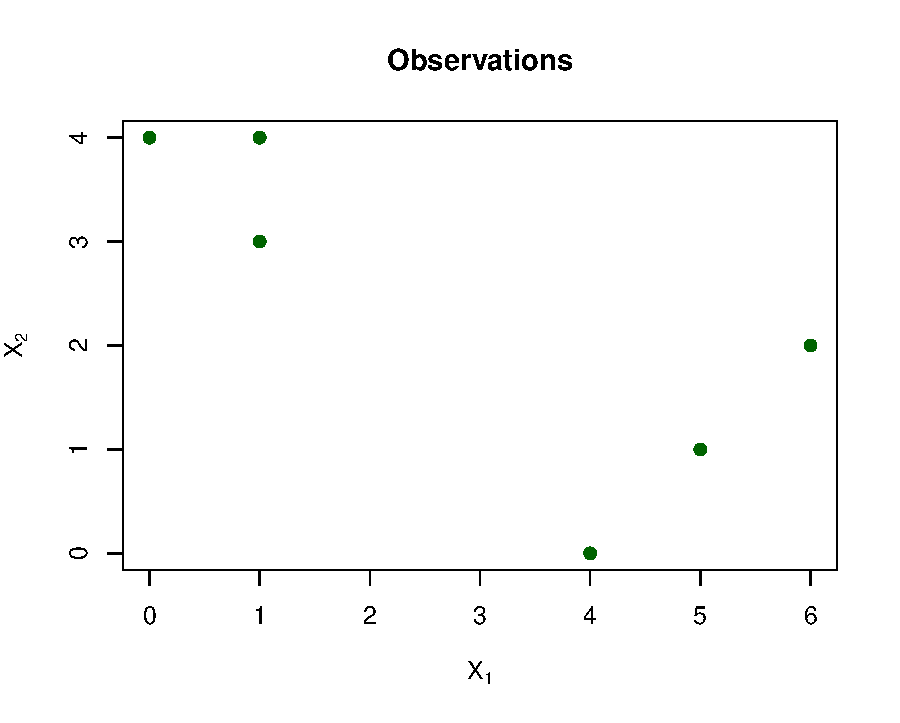
\includegraphics[width=0.75\linewidth]{Image/Prob1a.pdf}
\end{center}
\bigskip






\qnum{b}
The cluster labels are randomly assigned to each observations in \code{R} by using
\begin{minted}{r}
    sample.int(2, size = 6, replace = TRUE)
\end{minted}
One result is given in the table below. This result will be used in later calculations in this problem.
\begin{center}
  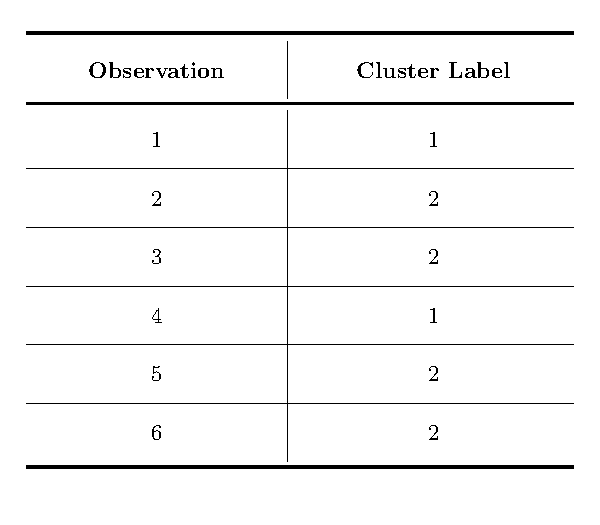
\includegraphics[width=4in]{Table/Table1.pdf}
\end{center}



\qnum{c}
In this case, the coordinates of the centroids are calculated as
\begin{itemize}
\item $
    \text{centroid 1} = 
    \left(
        \ds\frac{x_{11} + x_{41}}{2},
        \frac{x_{12} + x_{42}}{2}
    \right)
    = (3.0, 2.5)
$
\item $
    \text{centroid 2} = 
    \left(
        \ds\frac{x_{21} + x_{31} + x_{51} + x_{61}}{4},
        \frac{x_{22} + x_{32} + x_{52} + x_{62}}{4}
    \right)
    = (2.75, 2.25)
$
\end{itemize}
\bigskip



\qnum{d}
Using the coordinates of the centroids derived in (c), the distance between the $i^\text{th}$ observation $(x_{i1}, x_{i2})$ and the $j^\text{th}$ centroid $(c_{j1}, c_{j2})$ can be calculated by the following formula
\[
    \text{distance} = 
    \sqrt{
        (x_{i1} - c_{j1})^2 + (x_{i2} - c_{j2})^2
    }
\]

Applying this formula to all pairs of observation and centroid, I derived the following results. 

\begin{center}
  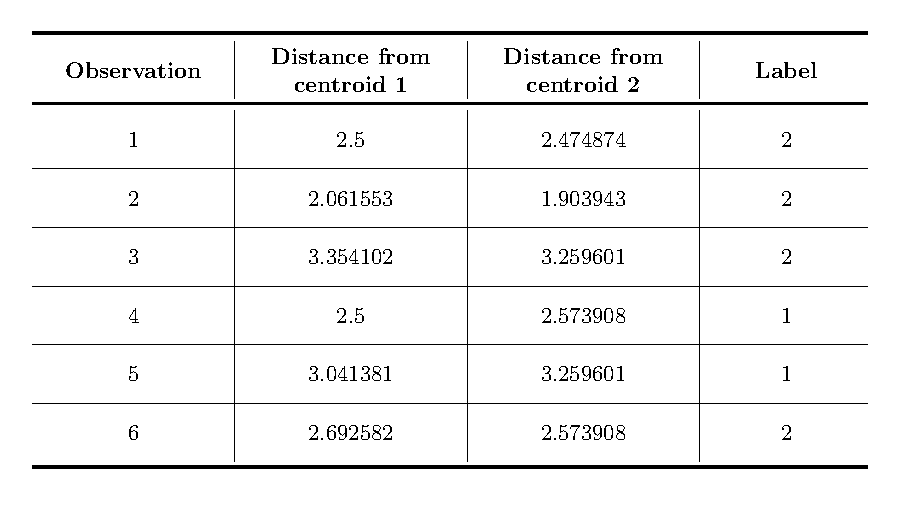
\includegraphics[width=6in]{Table/Table2.pdf}
\end{center}



\qnum{e}
I repeated the process and generated the following results


\begin{center}
  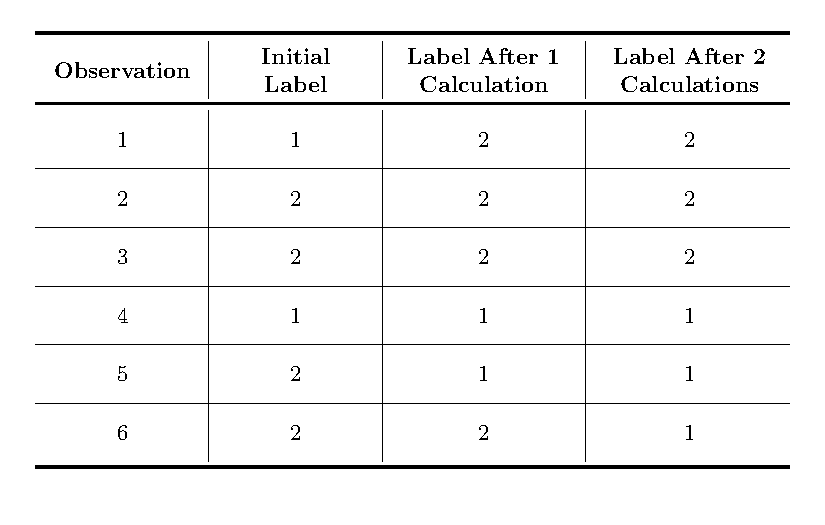
\includegraphics[width=5.5in]{Table/Table3.pdf}
\end{center}
%
The labels (or equivalently the assignments to clusters) stopped changing after 2 calculations.
\bigskip\bigskip 



\qnum{f}
The clustering result is shown in the the plot below. Green points represent observations in cluster 1 and orange points represent observations from cluster 2.
\begin{center}
  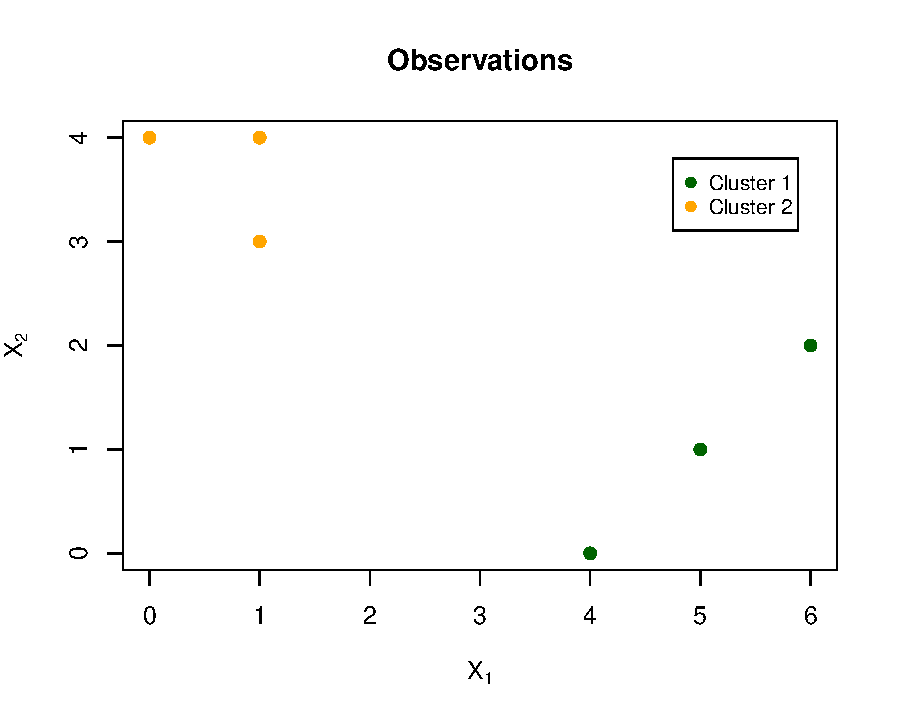
\includegraphics[width=0.75\linewidth]{Image/Prob1f.pdf}
\end{center}








\newpage
\section*{Problem 2 [20 points]} 

The pseudo-code for $k$-means and a running example of $k$-means on a small data set are provided above. Answer the following questions

\begin{enumerate}
  \item[2.1] Does $k$-means always converge? Given your answer, a bound on the iterate must be included. How is
its value determined?
  \item[2.2] What is the run-time of this algorithm?
\end{enumerate}
\sep 



\qnum{2.1}
$k$-means algorithm (the one given in the homework description) always converges. But it can converge very slowly. A theoretical (but trivial) upper bound on the number of iterations is $k^n$, which is the number of all possible clustering results with at most $k$ clusters.

In practice, the bound (usually) should be set to a much smaller number than the exponential upper bound (especially when $k$ and $n$ are large). 
Its value can be determined by running the algorithm on specific problems with specific machines and observing the run time. Then a reasonable value for the upper bound on iterations can be set according to the performance of the algorithm.
\bigskip


\qnum{2.2}
The run-time of the given $k$-means algorithm is $O(nkdi)$, where $n$ is the number of data points, $d$ is the dimension of data, and $i$ is the total number of iterations.

(The run-time is contributed by line 20-23, where in comparison, line 13-16 contributed $O(k)$, line 24-31 contributed $O(k^2i)$, and line 34 contributed $O(kdi)$.)

An upper bound on the run-time can be given as $O(k^{n+1}nd)$.
\bigskip




















\newpage 
\section*{Problem 3 [50 points]} 

 Implement Lloyd's algorithm for $k$-means (see algorithm $k$-means below)  in \textit{R} and call this program $C_k$. As you present your code explain your protocol for


\begin{enumerate}
  \item[3.1] initializing centroids
  \item[3.2] maintaining $k$ centroids
  \item[3.3] splitting centroids
  \item[3.4]  deciding ties
  \item[3.5] stopping criteria
\end{enumerate}
\sep 


\qnum{3.1}
In my implementation, the centroids are initialized by randomly labeling all the data points and then calculate the centroid of each cluster.

Specifically, for each data point, one label is randomly selected from the $k$ labels and assigned to that data point.

To make sure $k$ clusters are generated, after all data points are labeled, $k$ data points are drawn randomly from the $n$ data points and then labeled as \code{cluster 1}, \code{cluster 2}, $\cdots$, \code{cluster k}.
\bigskip 


\qnum{3.2-3.3}
To maintain $k$ centroids, I used the following splitting method.

In any iteration, once empty clusters form, they will be detected when new centroids are calculated (specifically when the means are taken). 
Then the number of empty clusters will be noted. Suppose there are $m$ empty clusters. The algorithm maintains $k$ clusters by the following steps.
\begin{enumerate}
    \item Randomly draw $m$ data points from all data points that do NOT belong to clusters with single points.
    \item Assign these $m$ data points to the $m$ empty clusters as their new centroids.
    
    \item Then proceed as usual and label all data points by using the newly derived $k$ centroids.
\end{enumerate}
\bigskip


\qnum{3.4}
In the situation of a tie, I did not add any special procedure. 
A data point will be assigned smaller label number whenever there is a tie in comparing distances.

This treatment will not add to the complexity of algorithm, and thus will be easy on run-time. Multiple runs with different initial conditions can help with possible bias generated.
\bigskip


\qnum{3.5}
For the stopping criteria, I observed the performance of my program on my machine and set the maximum number of iterations to 1000. 

Also, my program uses the average of the 2-norm in the changes of the centriods (see line 34 in the algorithm)
\[
  \code{change} = 
  \frac{1}{k}\sum_{j=1}^k\|c_{j}^{i-1} - c_j^i\|
\]
The tolerance $\tau$ is set to be $0.001$. This value allows my program to finish in reasonable time and produce a good result.





























\newpage  
\section*{Problem 4 [50 points]}
 
 In this question, you are asked to run  your program, $C_k$, against the Ringnorm and Ionosphere data sets and answer the following question. Click on the links to download the data sets.
 \begin{itemize}
 \item  \href{http://mldata.org/repository/data/viewslug/ringnorm-ida/}{Ringnorm Data Set}
 \item  \href{https://archive.ics.uci.edu/ml/datasets/ionosphere}{
Ionosphere Data Set }
 \end{itemize}
 
 
 
  Upon stopping, you will calculate the quality of the centroids and of the partition.  For each centroid $c_i$, form two counts (over Ionosphere Data Set)  :
  \begin{eqnarray*}
  g_i &\gets& \sum_{\delta \in c_i.B} [\delta.C ==\text{\quotes{g}}],\ \ \ \mbox{\rm good}\\
  b_i &\gets& \sum_{\delta \in c_i.B} [\delta.C = =\text{\quotes{b}}], \ \ \ \mbox{\rm bad}
  \end{eqnarray*}
  where $[x = y]$ returns 1 if True, 0 otherwise.  For example, $[2 = 3] + [0 = 0] + [34 = 34] = 2$
  
  The centroid $c_i$ is classified as good if $g_i > b_i$ and bad otherwise.  We can now calculate a simple error rate.    Assume $c_i$ is good.  Then the error is:
 \begin{eqnarray*}
 error(c_i) &=& \frac{b_i}{b_i + g_i}
 \end{eqnarray*}
 We can find the total error rate easily:
 \begin{eqnarray*}
 Error(\{c_1, c_2, \ldots, c_k\}) &=& \sum_{i=1}^k error(c_i)
 \end{eqnarray*}

Report the total error rates for $k = 2,\ldots 5$ for 20 runs each, presenting the results that are easily understandable.  Plots are generally a good way to convey complex ideas quickly. Discuss  your results.
\sep 


\qnum{1} 
The plot of total error rates for the Ringnorm Data Set is given below.
The green, orange, purple, and red dots represents total error rates from $k = 2,\ 3,\ 4, $ and 5 respectively. Each color has 20 dots, representing results from 20 runs.

\begin{center}
  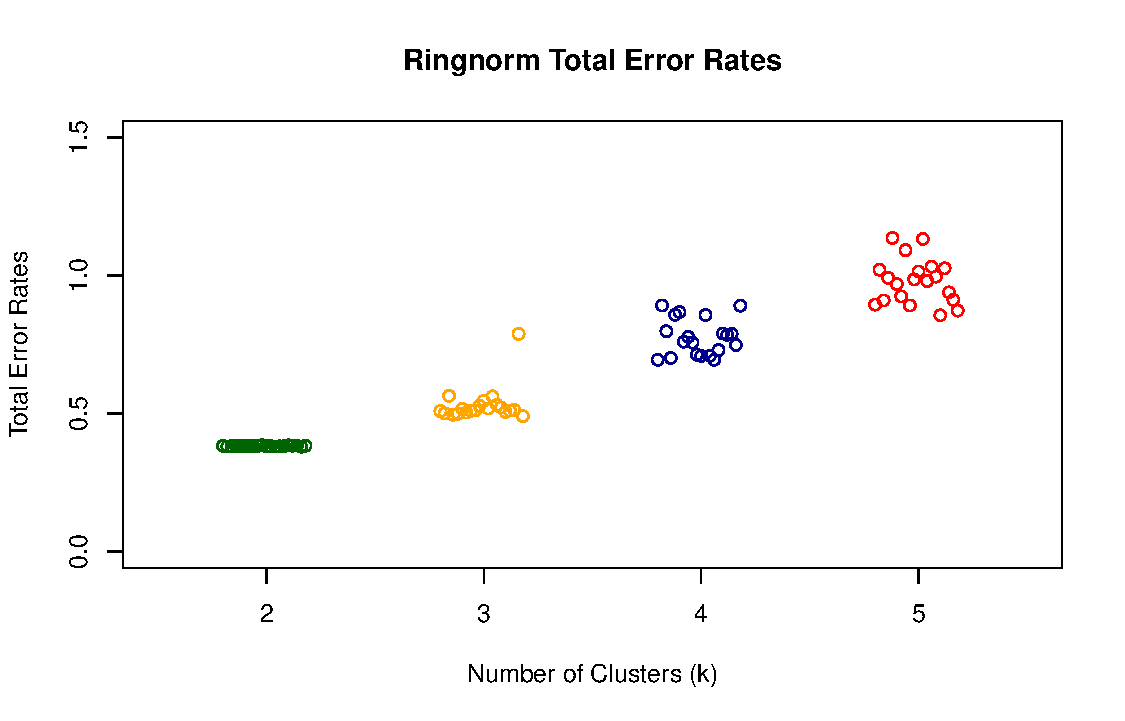
\includegraphics[width=0.9\linewidth]{Image/Prob4-ring.pdf}
\end{center}


\qnum{2}
The plot of total error rates for the Ionosphere Data Set is given below.
The green, orange, purple, and red dots represents total error rates from $k = 2,\ 3,\ 4, $ and 5 respectively. Each color has 20 dots, representing results from 20 runs.

\begin{center}
  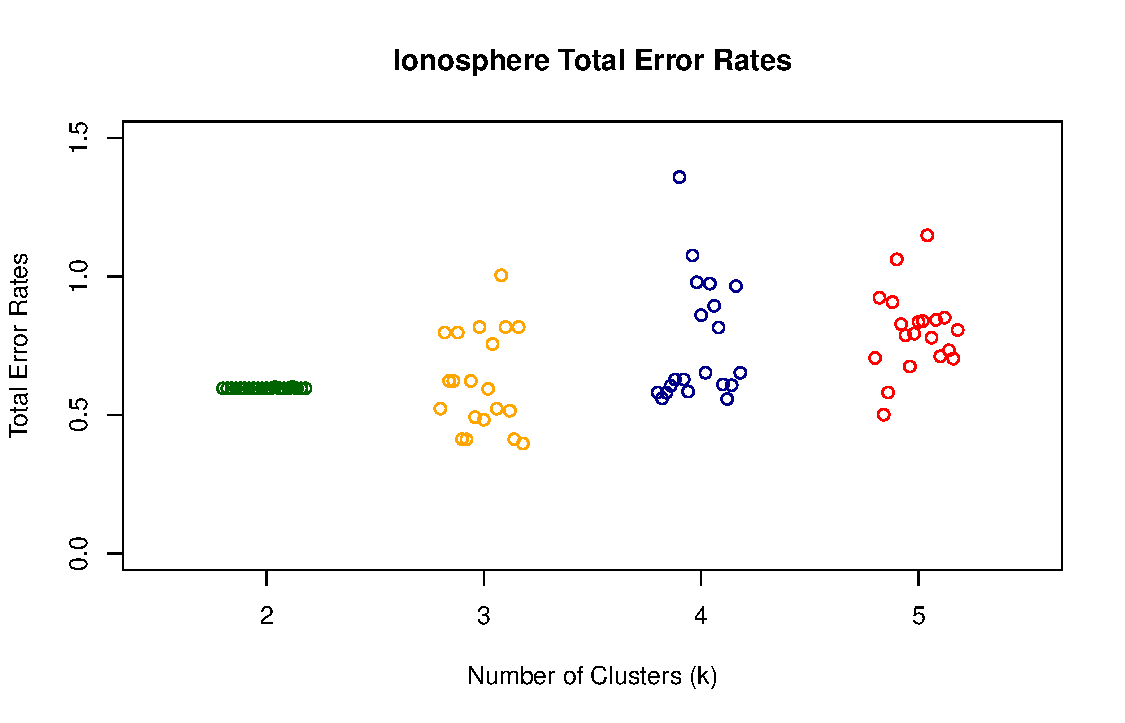
\includegraphics[width=0.9\linewidth]{Image/Prob4-iono.pdf}
\end{center}


\qnum{3} \textbf{Analysis of the results.}
From the two plots of total error rates, the following observations can be seen.
\begin{enumerate}
    \item In general, the error rates are not high, but not small as well. The average error rate in one cluster is around 20\% (see the plot for average error rates in one cluster below). This implies that the (Lloyd) $k$-means algorithm works for this data set, but does not cluster perfectly.
    \begin{center}
    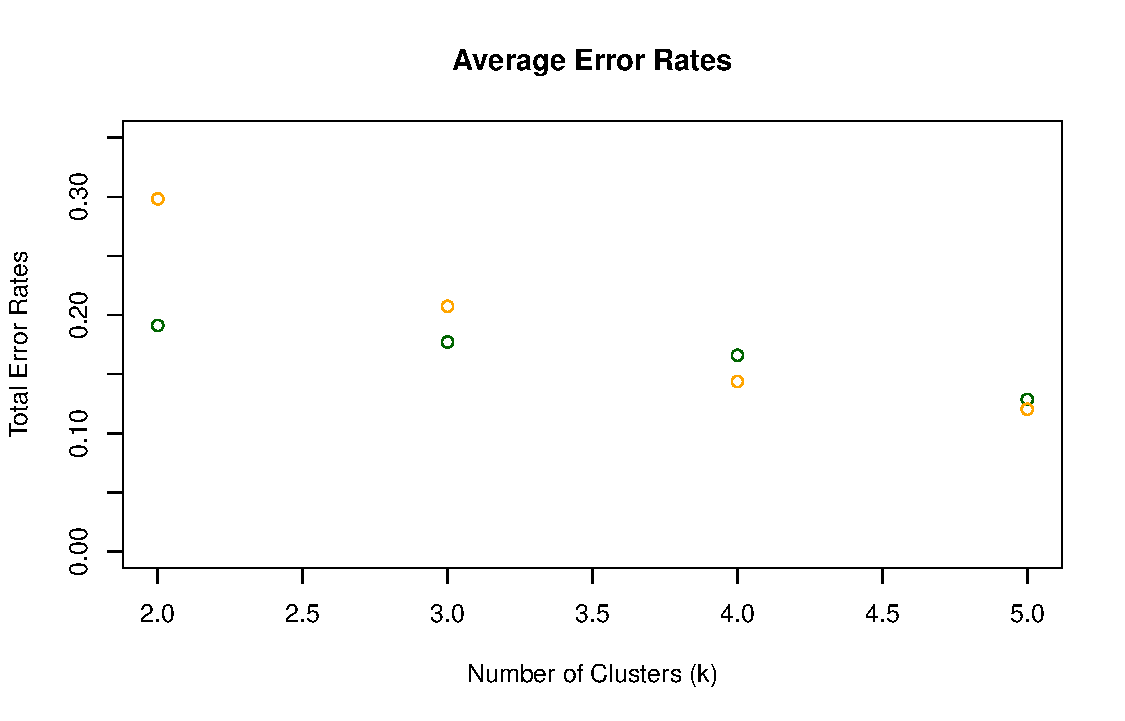
\includegraphics[width=0.9\linewidth]{Image/Prob4-aveErrRates.pdf}
    
    \parbox{0.75\textwidth}{\small \textit{In the plot, each dark green dot represents the average error rate in one cluster from the Ringnorm calculations. The orange dot represents the ones from the Ionosphere calculations.}}
    \end{center}

    \item The error rates for $k=2$ in calculations for both data set are very stable, indicating that there is high probability that only one local optimum exists, which is the global optimum (although another possibility is that the optimum is the only algorithm can converge to, which indicates flaws in the program, specifically in the initialization and tie-breaking methods). For the Ringnorm data, the error rates do not vary too much, whereas for the Ionosphere data, the error rates showed large variance. This indicates that many local solutions exist for Ionosphere Data Set problem and the solution is highly dependent on the initial conditions. 
    
\end{enumerate}

















\newpage 
 \section*{Problem 5 [50 points]} In this question, you are asked to make use of  the \href{https://stat.ethz.ch/R-manual/R-devel/library/stats/html/kmeans.html}{ R package for $k$-means implementation.} Elbow method is one of the techniques to decide the optimal cluster number.  Find the optimal number of clusters using elbow method for Ringnorm and Ionosphere data sets. Report your results in a plot as shown  \href{  https://www.r-bloggers.com/finding-optimal-number-of-clusters/}{
here} for  $2 \leq k \leq 10$. (The link includes an example.)
\sep 


We plot the total within-clusters sum of squares for $k = 2, 3, \cdots, 10$. 

\begin{center}
  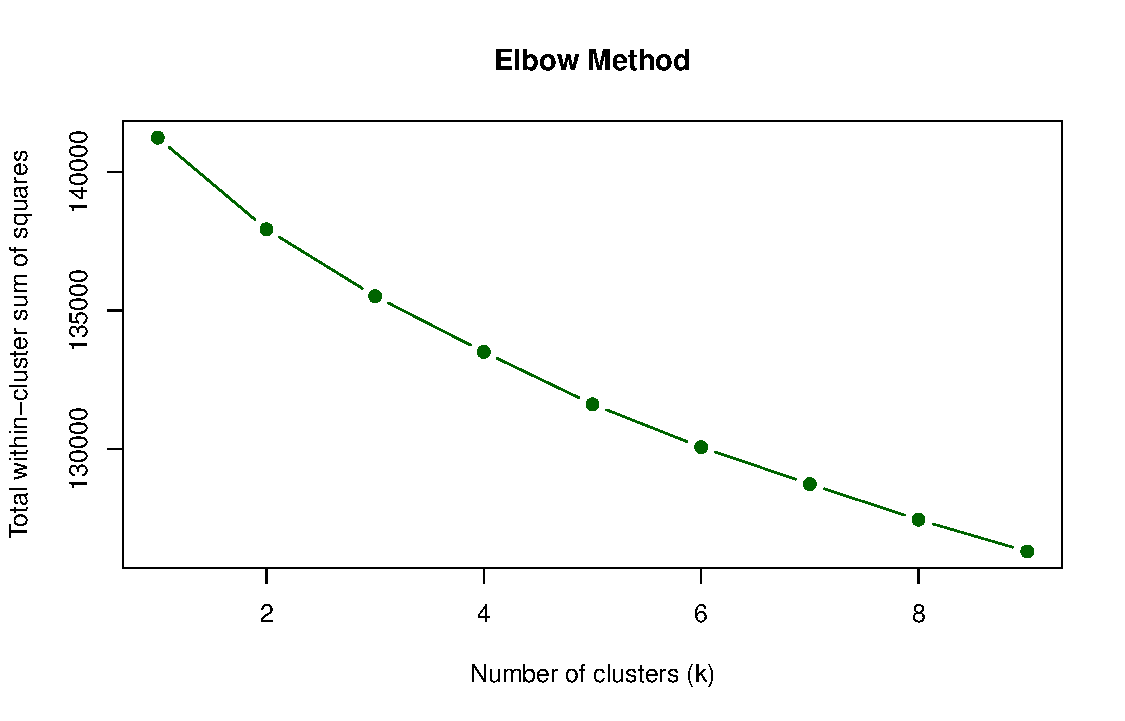
\includegraphics[width=0.9\linewidth]{Image/Prob5-elbow.pdf}
\end{center}
 
From the plot we can see that at $k=2$ (or $k=3$), the (between sum of squares) / (total sum of squares) ratio tends to change slowly and remain less changing as compared to other $k$'s. So $k=2$ or $k=3$ should be good choices for the optimal number of clusters.
 
 
 
 
 
 
 
 
 
 
 
\newpage
\section*{Problem 6 [20 points]}

Let $X \subset \mathbb{R}^n$  ($\mathbb{R}$ is the set of reals) for positive integer  $n>0$. Define a  distance $d: X \times X \rightarrow  \mathbb{R}_{\geq 0} $ as

\begin{equation*}
d(x,y) =  max\{|x_i - y_i|\}, \forall i\ 1\geq i \geq n
\end{equation*}

Is $d$ a metric?
\sep 

$d$ is a metric.
This can be shown by checking the 4 conditions in the definition of a metric.
\begin{enumerate}
    \item (\emph{Non-negativity}) Since $|x_i - y_i|\ge 0$ for all $i$, 
    \[
        d(x,y) = \max_{1\le i\le n}\{|x_i-y_i|\} \ge 0
    \]
    
    \item 
    \[\begin{aligned}
        &\ d(x, y) = 0 \\
        \Leftrightarrow&\ 
        \max_{1\le i\le n}\{|x_i-y_i|\} = 0\\
        \Leftrightarrow&\
        |x_i-y_i| = 0,\ \ 
        1\le i \le n\ \text{(Because $|x_i-y_i| \ge 0$ for all $i$)}\\
        \Leftrightarrow&\
        x_i = y_i,\ \ 
        1\le i \le n\ \\
        \Leftrightarrow&\ 
        x=y
    \end{aligned}\]
    
    \item (\emph{Symmetry})
    \[\begin{aligned}
        d(x,y) 
        =& \max_{1\le i\le n}\{|x_i-y_i|\}\\
        =& \max_{1\le i\le n}\{|y_i-x_i|\}\\
        =& d(y,x) 
    \end{aligned}\]
    
    
    \item (\emph{Triangle inequality})
    \begin{equation}\begin{aligned}
        d(x,y) + d(y,z) 
        =& \max_{1\le i\le n}\{|x_i-y_i|\} 
        + \max_{1\le i\le n}\{|y_i-z_i|\} \\
        \ge& \max_{1\le i\le n}\{|x_i-y_i|+|y_i-z_i|\}\\
        \ge& \max_{1\le i\le n}\{|x_i-z_i|\}\\
        =& d(x,z) 
        \label{201709152303}
    \end{aligned}\end{equation}
    The first inequality follows from the fact that
    \begin{equation}
        \max_{1\le i\le n}\{|a_i|\} + \max_{1\le i\le n}\{|b_i|\}
        \ge 
        \max_{1\le i\le n}\{|a_i| + |b_i|\}
        \label{201709152301}
    \end{equation}
    (A simple proof for this would be to see that $\max_{1\le i\le n}\{|a_i|\} + \max_{1\le i\le n}\{|b_i|\}\ge |a_j| + |b_j|$ for any $j$, by the definition of max. And then by taking max on $j$ on the right hand side, the inequality \eqref{201709152301} is proved.)
    
    The second inequality in \eqref{201709152303} follows by applying the triangle inequality on the real line, i.e.
    \[
        |x_i-y_i|+|y_i-z_i|\ge |x_i-z_i|
    \]
    
\end{enumerate}
\hfill Q.E.D.

















\newpage
\section*{Extra credit [90 points]}

This part is optional. 

\begin{enumerate}
\item[1]  Answer problem 4 using Breast Cancer Wisconsin Data Set. The data sets given in Problem 4 are clean. There are no missing values on those data sets. However, Breast Cancer Wisconsin Data Set has some missing values that must be removed to use with $k$-means algorithm. The data set can be found  \href{https://archive.ics.uci.edu/ml/datasets/breast+cancer+wisconsin+(original}{here} [30 points]

\item[2] The $k$-means algorithm provided above stops when centroids become stable (Line  34). In theory, $k$-means converges once SSE is minimized
\begin{eqnarray*}
SSE = \sum_{j}^k \ \ \smashoperator{ \sum_{x \in c_j.B}} ||\mathbf{x} - c_j.v||^2_2 \label{costfunt}
\end{eqnarray*} 
 
In this question, you are asked to use SSE as stopping criterion. Run $k$-means over Breast Cancer Wisconsin Data Set  and report the total SSE  in a plot for $k = 2,\ldots ,5$ for 20 runs each [30 points].

\item[3] Traditional $k$-means initialization is based on choosing values from a uniform distribution. In this question, you are asked to improve $k$-means through initialization.  \href{http://ilpubs.stanford.edu:8090/778/1/2006-13.pdf}{$k$-means ++} is an extended $k$-means clustering algorithm and induces non-uniform  distributions over  the data  that serve as  the initial centroids. Read the paper and discuss the idea in a paragraph.  Implement this idea to improve your $k$-means program. [30 points]
\end{enumerate}
\sep 


\qnum{1}
A plot on the total error rates is given below.
\begin{center}
  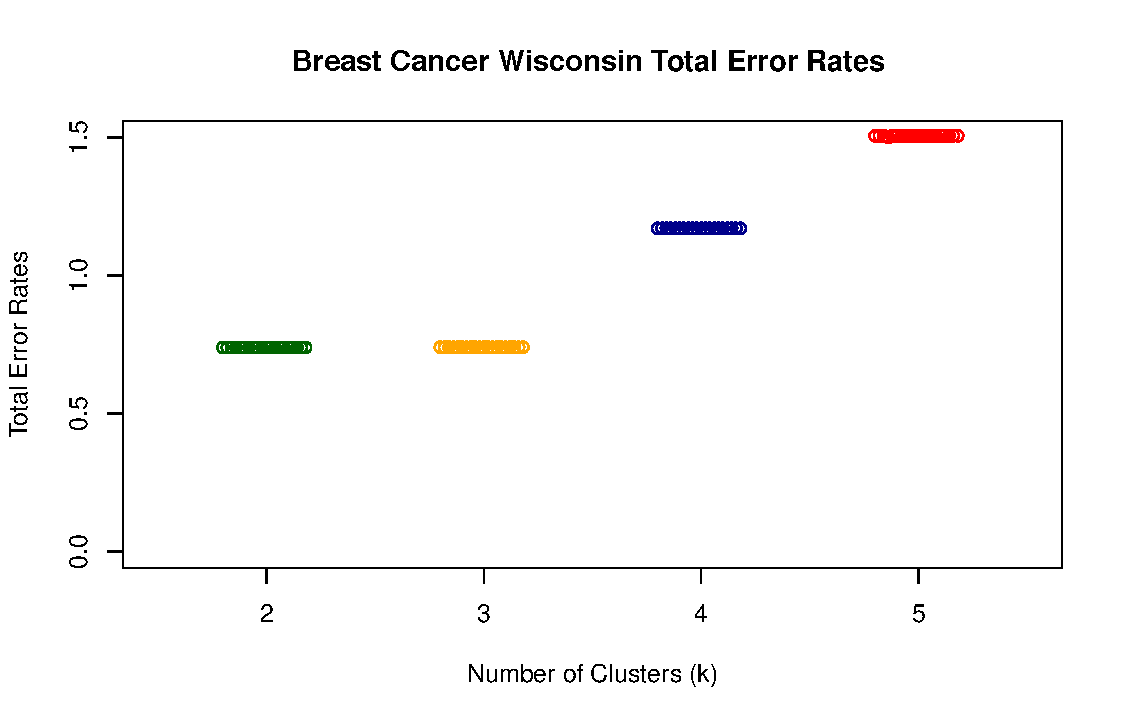
\includegraphics[width=0.9\linewidth]{Image/ProbEC1.pdf}
\end{center}

\textbf{Analysis of the result.}
In this data set, my Lloyd k-means program almost always converges to the same local optimum. This can be either because the program finds the true global optimum (the only local optimum), or the initialization method does not work well with this type of data set.
\bigskip


\qnum{2}
Using SSE in the stopping criterion, a plot of SSE is given below. 
\begin{center}
  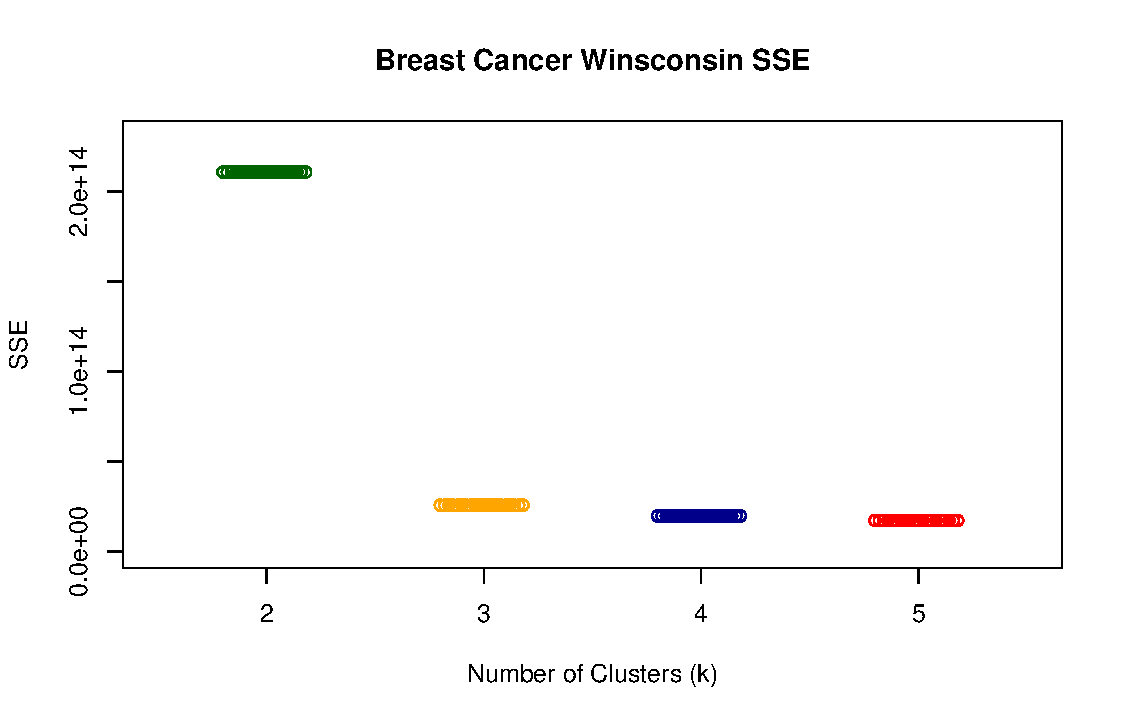
\includegraphics[width=0.9\linewidth]{Image/ProbEC2.pdf}
\end{center}







\qnum{3}
The $k$-means++ algorithm improves the original (Llyod) k-means algorithm on the initialization of centroids. Instead of choosing initial centroids randomly from uniform distribution, the $k$-means++ algorithm uses a different distribution, which is defined in the following way.

Let $D(x)$
denote the shortest distance from a data point to the closest center we have already chosen. First, one centroid is randomly chosen from a uniform distribution from $\Delta$ (the data set). Then we choose another centroid from a distribution where each data point $x$ has probability
\[
    \text{Pr}[\text{choose point } x] = \frac{D(x)^2}{\sum_{x\in \Delta} D(x)^2}
\]
Then update the probabilities and repeat the step until we have $k$ centroids in total. 

When choosing each centroid, $k$-means++ tries to make sure that points further away from the centroids already chosen have better chance of being selected. This in some way helps the algorithm to find better initial conditions to start with.

The algorithm is implemented by the \code{R} code in the file \code{ProbEC3.R}.
 

\end{document}


